\documentclass[conference, 11pt]{IEEEtran} 
\usepackage{verbatim}
\usepackage{multirow} \usepackage{enumerate}
\usepackage{amsmath,enumerate} \usepackage{amsthm}
\usepackage{algcompatible}
\usepackage{algpseudocode}
\usepackage{algorithm}
%\usepackage{algorithmic}
\usepackage{pstricks}
\usepackage{amssymb, latexsym}
\usepackage{xfrac}
\usepackage{mathtools}
\usepackage{graphicx}
\usepackage{subfig}
\DeclareGraphicsRule{*}{mps}{*}{}
\usepackage{listings}

%specific to this document only
\usepackage{pgfplots}
\usepackage{pgfplotstable}
\pgfplotstableread{plts/experiment8b1_av.tab}\averageone
\pgfplotstableread{plts/experiment8b2_av.tab}\averagetwo
\pgfplotstableread{plts/experiment8b3_av.tab}\averagethree
\pgfplotstableread{plts/experiment8b4_av.tab}\averagefour
\pgfplotstableread{plts/experiment9a_av.tab}\stepping
\pgfplotstableread{plts/experiment9a1_av.tab}\steppingone
\pgfplotstableread{plts/experiment9a2_av.tab}\steppingtwo
\pgfplotstableread{plts/experiment9a3_av.tab}\steppingthree
\pgfplotstableread{plts/experiment9a4_av.tab}\steppingfour
\pgfplotstableread{plts/experiment9b1_av.tab}\runningone
\pgfplotstableread{plts/experiment9b2_av.tab}\runningtwo
\pgfplotstableread{plts/experiment9b3_av.tab}\runningthree
\pgfplotstableread{plts/experiment9b4_av.tab}\runningfour
\pgfplotstableread{plts/experiment9b_av.tab}\running
\pgfplotstableread{plts/experiment9c_av.tab}\costcomp
\pgfplotstableread{plts/experiment9c1_av.tab}\costcompone
\pgfplotstableread{plts/experiment9c2_av.tab}\costcomptwo
\pgfplotstableread{plts/experiment9c3_av.tab}\costcompthree
\pgfplotstableread{plts/experiment8b1_rn.tab}\runsone
\pgfplotstableread{plts/experiment8b2_rn.tab}\runstwo
\pgfplotstableread{plts/experiment8b3_rn.tab}\runsthree
\pgfplotstableread{plts/experiment8b4_rn.tab}\runsfour
\pgfplotstableset{
  create on use/density/.style={
    create col/expr={\thisrow{nodes}+\thisrow{links}}}
    }
\pgfplotstableset{
  create on use/delta/.style={
    create col/expr={\thisrow{links}*2}}
    }
\pgfplotstableset{
  create on use/nodebylinks/.style={
    create col/expr={(\thisrow{nodes}*\thisrow{links})}}
    }
\pgfplotscreateplotcyclelist{three}{% 
  every mark/.append style={fill=teal}\\% 
  every mark/.append style={fill=green}\\% 
  every mark/.append style={fill=orange}\\% 
}
\pgfplotscreateplotcyclelist{four}{%
  every mark/.append style={fill=teal}\\%
  every mark/.append style={fill=green}\\%
  every mark/.append style={fill=orange}\\%
  every mark/.append style={fill=pink}\\%
}

%%%%%%%%%%%%%

\usepackage{pgf}
\usepackage{tikz}
\usetikzlibrary{decorations.pathmorphing} % LATEX and plain TEX when using Tik Z
\usetikzlibrary{positioning}
\usetikzlibrary{er}
\usetikzlibrary{automata}
\usetikzlibrary{shapes.geometric}
\tikzstyle{vx}=[draw,circle,fill=white,minimum size=2pt, inner sep=1pt, node distance=15mm]
\tikzstyle{ex}=[draw,rectangle,fill=white,minimum size=2pt, inner sep=3pt, node distance=15mm]
\tikzstyle{bup}=[semithick, decoration={bent, aspect=.3, amplitude=4}, decorate, ->, >=stealth]
\tikzstyle{bdn}=[semithick, decoration={bent, aspect=.3, amplitude=-4}, decorate, ->, >=stealth]
\tikzstyle{BUP}=[thick, decoration={bent, aspect=.3, amplitude=8}, decorate, ->, >=stealth]
\tikzstyle{BDN}=[thick, decoration={bent, aspect=.3, amplitude=-8}, decorate, ->, >=stealth]
\tikzstyle{MUP}=[thick, decoration={bent, aspect=.3, amplitude=16}, decorate, ->, >=stealth]
\tikzstyle{MDN}=[thick, decoration={bent, aspect=.3, amplitude=-16}, decorate, ->, >=stealth]
\tikzstyle{str}=[semithick, decorate, ->, >=stealth]
\tikzstyle{cr}=[draw, circle, fill=black!25,minimum size=150pt]

%styles for plots?
\tikzstyle{bls}=[blue, solid, mark=square*]
\tikzstyle{grt}=[red, solid, mark=*]
% \paperheight=11in \paperwidth=8.5in \textheight=9.0in
% \textwidth=6.5in \voffset=-.875in \hoffset=-.875in
\newenvironment{code} {\begin {quote}\begin{footnotesize}}
    {\end{footnotesize}\end{quote}}

% \oddsidemargin 0.0 in \evensidemargin 0.0 in
\newenvironment{enumeratealpha}
{\begin{enumerate}[(a{\textup{)}}]}{\end{enumerate}}

\theoremstyle{plain}
\newtheorem{lem-rule}{Rule}
\newtheorem{thm}{Theorem}
\newtheorem{lem}{Lemma}[thm]
\newtheorem{prop}{Proposition}[thm]
\newtheorem{lprp}{Proposition}[lem]
\theoremstyle{definition}
\newtheorem{defn}{Definition}[thm]
\newtheorem{dfn}{Definitions}[thm]
\newtheorem{ldef}{Definition}
\theoremstyle{remark}
\newtheorem{smy}{Summary}
\newtheorem{note}{Note}[thm]

%algorithms commands
\algblockdefx[Case]{Case}{EndCase} %
[1] [{\em var}] {{\bfseries case} {\em #1\ } } %
{{\bfseries end case}}%
\algcblockdefx[Case]{Case}{When}{EndCase}
[1] [{\em true}] {{\bfseries when} {\em #1\ }}
{{\bfseries end case}} %

\algblockdefx[TimesDo] {DoTimes}{EndTimes}
[1] [0] {#1 times {\bfseries do}}
{{\bfseries end do}}

%subalgorithms environment
\makeatletter
\newcounter{parentalgorithm}
\newenvironment{subalgorithms}{%
%  \refstepcounter{algorithm}%
  \floatname{algorithm}{Procedure}
  \protected@edef\theparentalgorithm{\thealgorithm}%
  \setcounter{parentalgorithm}{\value{algorithm}}%
  \setcounter{algorithm}{0}%
  \def\thealgorithm{\theparentalgorithm-\alph{algorithm}}%
  \ignorespaces
}{%
  \setcounter{algorithm}{\value{parentalgorithm}}%
  \ignorespacesafterend
}
\makeatother

%code environments
\usepackage{float}
 
\floatstyle{ruled}
\newfloat{codeblock}{thp}{lop}
\floatname{codeblock}{Example}

\lstnewenvironment{rubyblock} 
{\lstset{language=Ruby, basicstyle=\small, xleftmargin=10pt, numbers=left, numberstyle=\tiny, stepnumber=2, numbersep=5pt}}
{}
% text macros
\def\cI{{\mathcal I}} \def\cR{{\mathcal R}} \def\cE{{\mathcal E}}
\def\cC{{\mathcal C}} \def\cF{{\mathcal F}} \def\cU{{\mathcal U}}
\def\cH{{\mathcal H}} \def\cD{{\mathcal D}} \def\cB{{\mathcal B}}
\def\cQ{{\mathcal Q}} \def\cV{{\mathcal V}} \def\cS{{\mathcal S}}
\def\cG{{\mathcal G}} \def\cA{{\mathcal A}} \def\cO{{\mathcal O}}
\def\cW{{\mathcal W}} \def\cL{{\mathcal L}} 

\def\bI{{\mathbb I}} \def\bO{{\mathbb O}}
\def\bC{{\mathbb C}} \def\bM{{\mathbb M}}
\def\bId{{$\mathbb I$}} \def\bOd{{$\mathbb O$}}
\def\bCd{{$\mathbb C$}} \def\bMd{{$\mathbb M$}}

\def\cId{{$\mathcal I$}} \def\cRd{{$\mathcal R$}} \def\cEd{{$\mathcal E$}} 
\def\cCd{{$\mathcal C$}} \def\cFd{{$\mathcal F$}} \def\cUd{{$\mathcal U$}} 
\def\cHd{{$\mathcal H$}} \def\cDd{{$\mathcal D$}} \def\cBd{{$\mathcal B$}} 
\def\cQd{{$\mathcal Q$}} \def\cVd{{$\mathcal V$}} \def\cSd{{$\mathcal S$}} 
\def\cGd{{$\mathcal G$}} \def\cAd{{$\mathcal A$}} \def\cOd{{$\mathcal O$}}
\def\cWd{{$\mathcal W$}} \def\cLd{{$\mathcal L$}}

\bibliographystyle {IEEEtranS}

\begin{document}
\title{Distributed Vertex Cover and Network Lifetime Algorithms in Graphs} 

\author{\IEEEauthorblockN{J. Paul Daigle}
\IEEEauthorblockA{Department of Computer Science\\
Georgia State University\\
Atlanta, Georgia 30303\\
Email: jdaigle1@student.gsu.edu}
}

\maketitle

\begin{abstract}
  Target coverage in a sensor network can be easily modeled as a vertex covering problem. This paper explores the relationship between the Minimum Weighted Vertex Cover problem and the Network Lifetime problem. We present new algorithms for both MWVC and NL and test their performance against existing algorithms. We find that the algorithms that perform well for MWVC also perform well for NL.
\end{abstract}
\section{Introduction}
``Macroscopes'' composed of a network of wireless sensors are a valuable research tool in several science and security domains~\cite{1098925,990703}. Because such sensors have limited data processing capacities and limited battery life, it is important to use sensors efficiently. A common problem in sensor networks is the area coverage problem, which concerns the ability of the network to record data over an area or areas of interest. If the sensors are installed in some location where batteries can be replaced and the properties of the network are understood before deployment, this is not a difficult problem. However, sensor networks can also be randomly distributed in areas that are difficult to reach. In that case it is advantageous to have local, distributed algorithms to solve problems like area coverage.

Vertex Cover is a problem that is related to Target or Area coverage. Section~\ref{sec:area-vertex} presents a proof that the area coverage problem in a homogenous sensor network is equivalent to the vertex cover problem in the hypergraph. A graph is a special case of hypergraph, a 2-uniform hypergraph, so the argument extends to graphs. Section~\ref{sec:life-depend} presents a rationale for examining the Minimum Weighted Vertex Cover (MWVC) problem in relation to network lifetime. Other problems in biology, communication, and circuit design can also be formulated as instances of MWVC.

It has been shown that a constant approximation of MWVC cannot be found by a distributed algorithm in a constant number of rounds.\cite{1011811} We present a distributed two-approximate algorithm to solve MWVC in an expected running time of $O(logn)$, based on the sequential algorithm of Gonzalez.\cite{Gonzalez1995129} This is not the first such algorithm to appear in the literature, but there are implementation advantages to our approach.

Because of the relationship between Vertex Cover and Area Cover, we consider whether strategies that reduce the minimum weighted vertex cover can be used to increase network lifetime by considering weight as a measure of battery life. Accordingly, we introduce a new Algorithm for Weighted Vertex Cover with constant run time and consistent 2-approximate performance and compare its performance in extending network lifetime versus the one-hop algorithm of Prasad and Dhawan \cite{Dhawan:hipc-09}. 

All of the distributed algorithms described are assumed to be running on a message passing model, the compute nodes are mapped to the vertexes of the graph, and the edges of the graph represent viable paths for communication between nodes. 

\section{Prior Work}

\section{Coverage Problems}
The coverage problems in this paper are common coverage problems which are known to be NP-Complete. For convenience, the problem definitions are provided here.
\subsection{Problem Definitions}
\subsubsection{Minimum Vertex Cover (MVC)}
\label{sub:mvc}
Given an undirected Graph $G(V,E)$, a {\em Vertex Cover} of $G$ is a set of vertices $V'$ such that for each edge $e_{u,v} \in E$, $u \in V'$ or $v \in V'$. The Minimum Vertex Cover Problem is to find the smallest possible vertex cover of $G$.

\subsubsection{Minimum Weighted Vertex Cover (MWVC)}
\label{sub:mwvc}
Given an undirected Graph $G(V,E)$, where each $v \in V$ has a positive weight $w(v)$, minimize $\sum_{v \in V'} w(v)$.

%\subsubsection{Minimum (Weighted) Vertex Cover of a Hypergraph}

%Given a Hypergraph $G(V,E)$, with vertices $v \in V$ and hyperedges $e_{v_1...v_n}$, a vertex cover of $G$ is a set $V'\: | \: \forall e \in E,\quad \exists v \in V'\: |\: v \in e$. The minimum vertex cover and minimum weighted vertex cover are as described in sections~\ref{sub:mvc} and ~\ref{sub:mwvc}

\subsubsection{Target Coverage}
\label{sub:tar-cov}

\subsection{Area Cover as Vertex Cover}
\label{sec:area-vertex}
The area coverage problem in sensor networks has been shown to be equivalent to target coverage.\cite{IPDPS.2008.45361} This can be extended to the vertex cover problem in Hypergraphs. Intuitively, there is an obvious relationship between the collection of vertices that make up a given edge and the collection of sensors that cover a given target.  Theorem~\ref{thm:equiv} formally expresses this equivalency.

\begin{thm}
  For a given network $N(S,T)$ with sensors $s\in S$ and targets $t\in T$, there exists an equivalent hypergraph $G(V,E)$ such that any solution to the target coverage problem in $N$ is a vertex cover in $G$.
\label{thm:equiv}
\end{thm}
\begin{proof}[Proof of Theorem~\ref{thm:equiv}]
\label{prf:equiv}
\begin{defn}
For $N(S,T)$, define set of all sensors which can cover a target as $c(t_i) = \{s \in S | s \text{\ covers\ } t\}$.  For example, if sensors $s_1, s_4, s_7$ are all of the sensors that cover $t_3$, $c(t_3) = \{s_1, s_4, s_5\}$. \label{defn:network}
\end{defn}
\begin{defn}Construct the equivalent hypergraph $G(V,E)$, as $V \cong S$ and $E$ is isomorphic to the set of hyper edges $c(t_i)$, for all $t_i \in T$. 
\label{defn:graph}
\end{defn}

To be shown: if $S' \subset S$ is a solution for target coverage in $N$, $S'$ is a vertex cover of $G$. 

We proceed by direct proof. Let us define $S'\subset S$ such that $S'$ is a target cover of $N$. If $S'$ is a target cover, we know by definition~\ref{defn:graph} that there is an isomorphic set $V'$ in $G$. It is to be shown that $V'$ is a vertex cover in $G$.

By the definition of a target cover, we know that:
\begin{equation}
\forall t \in T, \exists s \in S' | s \in c(t)
\label{eqn:tcover}
\end{equation}
That is, for every target, there is a sensor in $S'$ that covers that target.

By substituting isomorphic sets, equation~\ref{eqn:tcover} implies that:
\begin{equation}
\forall t \in T, \exists v \in V', e \in E | v \in e
\label{eqn:tvbridge}
\end{equation}

Since we know by definition~\ref{defn:network} that each target has a unique set of neighboring sensors covering it, which is isomorphic to one and exactly one edge, we can substitute again, yielding:
\begin{equation}
\forall e \in E, \exists v\in V' | v \in e
\end{equation}

Therefore $V'$ must be a vertex cover of $G$.  
\end{proof}


It follows from the proof that if a target cover is minimal for the sensor network, the equivalent cover in the hypergraph is minimal to that graph. Similarly, a MVC of the isomophic hypergraph is a minimum target cover for the sensor network. It also follows that target coverage is equivalent to vertex cover in a graph, because a graph is a 2-cardinal hypergraph.

\section{Algorithms}
\label{sec:algorithms}

\subsection{Maximal Matching Algorithm for Minimum Weighted Vertex Cover}
Algorithm~\ref{alg:dgmm} is our distributed implementation of the 2-approximate minimum weighted vertex cover algorithm presented by Gonzalez.\cite{Gonzalez1995129} The Gonzalez algorithm proceeds by selecting each edge in turn and choosing one of the endpoints of that edge to add to the cover. The sequential algorithm goes through each edge in turn, adding vertexes when necessary. Each edge, as examined, is assigned a weight according to equation~\ref{eqn:gmm}. If the weight of a vertex is equal to the sum of it's incident edge weights, that vertex is added to the cover. 

\begin{equation}
  \label{eqn:gmm}
  w(e(u,v)) = min 
  \begin{dcases} 
    w(u) - \sum_{i \ne v} w(e(u,i)) \\
    w(v) - \sum_{i \ne u} w(e(i,v)) 
  \end{dcases}    
\end{equation}

The distributed version of the algorithm chooses some disjoint set of edges and performs exactly the same calculations. The precise method of choosing edges and updating weights is given in Algorithm~\ref{alg:dgmm}. The general progress of the algorithm is defined by the automata in Figure~\ref{fig:dgmm-auto}. Each node begins in the \cCd state, and chooses to either send invitations (\cId), or listen for invitation (\cLd). Nodes in the \cId state choose one neighbor to send an invitation to and wait for a response \cWd, and nodes in the \cLd state choose one invitation to accept, which is sent in the response state \cRd. All nodes that have formed a pair in this manner then update their status (\cUd) and (\cEd) exchange data with their neighbors. Nodes that have chosen to turn on or off move to the done state (\cDd).  

\begin{figure}[htp]
  \caption{DGMM Automata}
  \begin{center}
  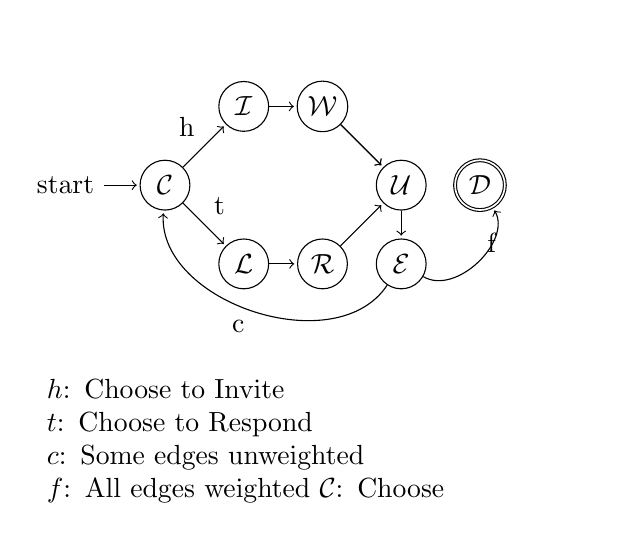
\begin{tikzpicture}[shorten >=1pt,node distance=1cm,on grid,auto, bend angle=75, every state/.style={scale=1, minimum size=18pt, inner sep=2pt}]
    %\draw [help lines] (0,-2) grid (4,2);
    \path [help lines] (0,-2) grid (4,2); 
    \node [state, initial]   (C)          {\cCd};
    \node [state] (I)            at (1,1) {\cId};
    \node [state] (L)            at (1,-1) {\cLd};
    \node [state] (W)            at (2,1)       {\cWd};
    \node [state] (R)            at (2,-1)       {\cRd};
    \node [state] (U)            at (3,0) {\cUd};
    \node [state] (E)            at (3,-1)       {\cEd};
    \node [state, accepting] (D) at (4,0)   {\cDd};

    \path [->] (C) edge              node {h} (I)
                   edge              node {t} (L)
               (L) edge              node {} (R)
               (I) edge              node {} (W)
               (W) edge              node {} (U)
               (R) edge              node {} (U)
               (U) edge              node {} (E);
    \path [->] (E) edge [bend right] node [above right] {f} (D);
    \path [->] (W) edge              node {} (U);
    \path [->] (E) edge [bend left]  node {c} (C);


      \node [text width=7cm] (key) at (2, -3.25) {
	$h$: Choose to Invite \hspace{4cm}
        $t$: Choose to Respond\hspace{4cm}
        $c$: Some edges unweighted\hspace{5cm}
	$f$: All edges weighted
	$\cC$: Choose 
	}; 
  \end{tikzpicture}
  \end{center}
  \label{fig:dgmm-auto}
\end{figure}


Vertex pairs are able to assign a weight to the edge between them independently, and therefore decide whether or not to join the cover. During the \cEd stage neighboring vertexes are able to update some of their own edge weights. 

\begin{algorithm}
\caption{Distributed Weighted Vertex Cover}
\begin{algorithmic}
\Require {$G(V,E)$: a graph}
\ForAll {$v_u \in V$ in parrallel}
\State $S_u \leftarrow False$
\State state $\leftarrow$ Choose
\Repeat
\State Broadcast $S_u$
\If {$S_v = True$ for $v_v$ incident to self}
\State Set Weight $e_{u,v} \leftarrow 0$
\EndIf
\If {state = Choose}
\State {Choose A State (Invite, Listen)}
\ElsIf {state = Invite}
\State {Select an unweighted edge, $e_{u,v}$}
\State {Broadcast an Invitation to $v_v$}
\State {state $\leftarrow$ Wait}
\ElsIf {state = Listen}
\State {Collect Invitations}
\State {state $\leftarrow$ Respond}
\ElsIf {state = Wait}
\State {Collect Responses}
\If {Response Matches Invitation}
\State {Update Weight $e_{u,v}$}
\If {$\sum_{w_e} e incident v_u = w_u$}
\State $S_u \leftarrow true$
\EndIf
\EndIf
\State {state $\leftarrow$ Choose}
\ElsIf {state = Respond}
\State Choose Invitation, Broadcast Response
\State {Update Weight $e_{u,v}$}
\If {$\sum_{w_e} e incident v_u = w_u$}
\State $S_u \leftarrow true$
\EndIf
\State {state $\leftarrow$ Choose}
\EndIf
\Until {$S_u = true$ OR $S_v = true$ for all $v_v$ incident $v_u$}
\EndFor
\end{algorithmic}
\label{alg:dgmm}
\end{algorithm}

\subsection{Proof of 2-Approximation}
The sequential version of Algorithm~\ref{alg:dgmm} has been shown to be 2-approximate for any ordering of edges. The distributed version can never select contiguous edges in a single round, as each node can form at most one partnership in a round. Because The simultaneous selection of vertexes to join the cover based on disjoint edges is exactly equivalent to the sequential selection of vertexes by selecting each edge under consideration in turn.\footnote{This algorithm could therefore also be used to provide an edge coloring in approximately the same time, equivalent to a greedy linear algorithm.}


\section{Dependency Graph}
\label{sec:life-depend}
Target Coverage and Minimum Weighted Vertex Cover are both NP-Complete problems. It has also been proved that MWVC cannot be approximated to a constant factor locally within any constant number of communication rounds~\cite{1011811}, and as we have shown this limitation must apply to target coverage as well. The Dependency Graph is a heuristic framework for such problems~\cite{IPDPS.2008.45361}. It has been shown to produce good results when applied to the Lifetime Maximization problem in sensor networks~\cite{978-3-540-89894-8_26}.

The framework applies to problems where local solutions can be combined to form a feasible global solution. The essential steps of the framework are: 
\begin{enumerate}
\item Establish that combined local solutions lead to a feasible global solution
\item Model the state space of the local solutions
\item Determine a priority heuristic for local solutions
\item Design a reasonable negotiating strategy between neighbors
\end{enumerate} 
A detailed description of each of these steps can be found in~\cite{IPDPS.2008.45361}.

The application of the framework relies on dependencies between local solutions. In the case of the MWVC problem, there are several approaches that can be taken to determine what a local solution is. The simplest approach is to have each vertex only consider edges incident to itself. Naively, each vertex would have exactly two local solutions, the cover containing itself and the cover containing all of its neighbors. This would be insufficient for allowing for any negotiation between neighbors, as shown in Figure~\ref{fig:negprob}. If each vertex can {\em only} choose either itself or all its neighbors, the feasible solutions give weights of 34 and 29, but the optimal solution for that graph is 13. Other graphs could be constructed in which no solution would be possible with these constraints, such as a 4-clique. So even for this simple case, a large number of possible covers have to be considered. The number of possible local covers for a vertex of degree $\Delta$ is $\sum_{i=0}^\Delta \binom{\Delta}{i}$.

\subsection{Dependency Graph}
Given a Weighted Graph $G(V,E)$, a {\em Dependency Graph} $H(S,D)$ for $v \in V$ is defined by local solutions $s \in S$ and dependencies $d_{u,v} \in D$ between those solutions. In the case of the MWVC, each solution is made up of a set of vertices that cover the edges incident to $v$. The goal is to use the local solutions to build $\cC$, a vertex cover of $G$. The initial dependency graph for each vertex $v$ consists of the set containing the vertex $\{v\}$, and the set containing the neighbors of $v$, $\{n_v)\}$. 

\subsection{Prioritizing Local Solutions}

Given two local covers $c_1, c_2$, we define the degree of a cover ($w(c)$) as $\sum w(v)\:|\: v \in c, v \notin \cC$.  

\subsection{Negotiation Strategies}
Initially, each vertex $v$ is only aware of two solutions, the solution containing itself $s_s$ and the solution containing all of its neighbors $s_n$, which have no dependencies between them. In order to ensure 2-approximation, $v$ can only safely join $\cC$ if its own weight $w_v$ is at most half of the cumulative weight of all $w_u, u \in s_n $. If that condition cannot be met, then a vertex can join $\cC$ if it is the smallest node in it's local neighborhood not in $\cC$. A vertex that cannot meet either of these conditions waits for the next round. 

Some nodes will turn on, and in doing so will create new covers for their neighbors. At the beginning of each round, each vertex notes whether any vertexes in $s_n$ have joined $\cC$, and if so, it creates a new solution $s$ composed of itself and those vertexes. This solution will have a dependency to both $s_s$ and $s_n$, and the decision criteria can be applied to this new solution. 

\subsection{Partial Cover Dependency Graph}

The number of local covers increases as a function of the density of the local neighborhood. If $\Delta$ is small, this is not a problem, but as $\Delta$ increases the number of potential local covers increases rapidly. The Partial Cover Dependency Graph samples this exponential space and reduces the number of solutions to $\Delta$. A given vertex can only see two covers for it's own edges: the cover containing itself, and the cover containing all of its neighbors. The partial cover dependency graph samples the solution space based on what vertexes would have to be on if either of these two covers were off. 

\subsubsection{Construction of the PCDG}

Given a graph $G(V,E)$, for each vertex in $V$ we can define a partial cover dependency graph consisting of the {\em partial cover pair} $\cC_v, \cC_{n(v)}$ for v, and the partial cover pair for each neighbor of v. Given a node $v \in V$, $\cC_v$ consists of v and its two-hop neighbors, while $\cC_{n(v)}$ consists of $v$'s one-hop neighbors. For clarity, we define terms below.

\begin{defn}
One-hop Neighbor of $v$ : $u \in V \mid \exists e(u,v) \in E$
\end{defn}

\begin{defn}
Two-hop Neighbor of $v$ : $u \in V \mid \exists e(u,w) \in E \land \exists e(w,v) \in E \land \neg\exists e(u,v) \in E$
\end{defn}

\begin{defn}
$N_v$ : The set of one-hop neighbors of $v$
\end{defn}
\begin{defn}
$N_v^2$ : The set of two-hop neighbors of $v$
\end{defn}

\begin{defn}
$\cC_v$ : $\{v\} \cup N_v^2$
\end{defn}

\begin{defn}
$\cC_{n(v)}$ : $N_v$
\end{defn} 

\begin{defn}
Partial Cover Dependency Graph of $v$ : a graph $H(C,F)$ such that \begin{align*}& 1. C = \{\cC_v, \cC_{n(v)}\} \cup \{\cC_u, \cC_{n(u)}\} \forall u \in N_v\\ & 2. \exists f(c_1, c_2) \in F \iff \exists u \in V \mid u \in c_1 \land u \in c_2\end{align*}.
\end{defn} 

After constructing $H$, each cover is assigned a {\em weight} and a {\em degree}. The weight of a cover is defined as the sum of the weight of the vertexes in that cover, and the degree is defined by the number of edges for that cover. Figure~\ref{fig:pcdg} shows a graph and the corresponding partial cover dependency graph of a vertex in that graph.

\begin{figure}[htp]
  \begin{center}
  \subfloat[Weighted Graph $G$]
  {  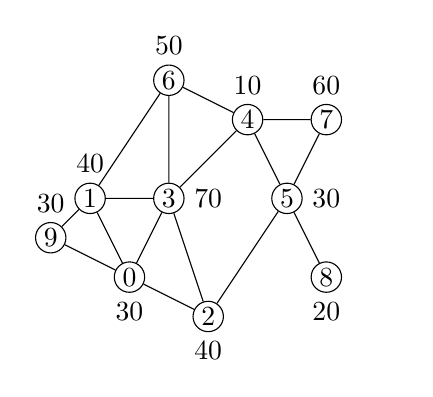
\begin{tikzpicture}
%      \draw [help lines] (0,-2) grid (4,2);
      \path [help lines] (0,-2) grid (4,2); 
      \node [vx, label=below:30]  (0) at (.5,-1) {0};
      \node [vx, label=above:40] (1) at (0, 0) {1};
      \node [vx, label=below:40] (2) at (1.5,-1.5) {2};
      \node [vx, label=right:70] (3) at (1, 0) {3};
      \node [vx, label=above:10] (4) at (2, 1) {4};
      \node [vx, label=right:30] (5) at (2.5, 0) {5};
      \node [vx, label=above:50] (6) at (1, 1.5) {6};
      \node [vx, label=above:60] (7) at (3, 1) {7};
      \node [vx, label=below:20] (8) at (3,-1) {8};
      \node [vx, label=above:30] (9) at (-.5,-.5) {9};
      \path [draw] 
      (0) -- (1)
      (0) -- (2)
      (0) -- (3)
			(0) -- (9)
      (1) -- (3)
      (1) -- (6)
			(1) -- (9)
      (2) -- (3)
      (2) -- (5)
      (3) -- (4)
      (3) -- (6)
      (4) -- (5)
      (4) -- (6)
      (4) -- (7)
      (5) -- (7)
      (5) -- (8);
    \end{tikzpicture}
}
  \\
  \subfloat[PCDG for Vertex 7]{
    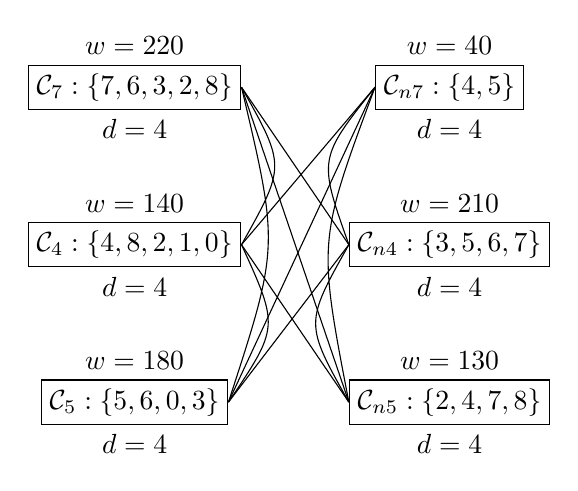
\begin{tikzpicture}
%      \draw [help lines] (0,-3) grid (6,3);
     \path [help lines] (0,-2) grid (4,2);
      \node [ex, label={above: $w=220$}, label={below: $d=4$}] (C7) at (1,2) {$\cC_7: \{7,6,3,2,8\}$};
      \node [ex, label={above: $w=40$}, label={below: $d=4$}] (CN7) at (5,2) {$\cC_{n7}: \{4,5\}$};
      \node [ex, label={above: $w=140$}, label={below: $d=4$}] (C4) at (1,0) {$\cC_4: \{4,8,2,1,0\}$};
      \node [ex, label={above: $w=210$}, label={below: $d=4$}] (CN4) at (5,0) {$\cC_{n4}: \{3,5,6,7\}$};
      \node [ex, label={above: $w=180$}, label={below: $d=4$}] (C5) at (1,-2) {$\cC_5: \{5,6,0,3\}$};
      \node [ex, label={above: $w=130$}, label={below: $d=4$}] (CN5) at (5,-2) {$\cC_{n5}: \{2,4,7,8\}$};

      \path [draw] 
      (C7.east) -- (CN5.west)
      (C7.east) -- (CN4.west)
      (CN4.west) -- (C5.east);
      \path [draw, decoration={bent, amplitude=16}, decorate]
      (C7.east) -- (C5.east)
      (C7.east) -- (C4.east)
      (C4.east) -- (C5.east);
      \path [draw]
      (CN7.west) -- (C5.east)
      (CN7.west) -- (C4.east)
      (CN5.west) -- (C4.east);
      \path [draw, decoration={bent, amplitude=-16}, decorate]
      (CN7.west) -- (CN5.west)
      (CN7.west) -- (CN4.west)
      (CN4.west) -- (CN5.west);
    \end{tikzpicture}
  }
  \end{center}
  \caption{Partial Cover Dependency Graph}
  \label{fig:pcdg}
\end{figure}


\subsubsection{PCDG Algorithm}

\subsection{Redundancy Checking}

When vertexes make local decisions to join a cover in constant time, it is difficult to judge whether any neighbor will also decide to join the cover. In some cases, this leads to vertexes joining the cover which can be subsequently removed while still retaining full coverage. Removing these nodes will certainly reduce the total weight of the cover, and may also increase the potential lifetime of the network. We therefore implement a {\em redundancy checking} algorithm for Vertex Cover. Figure~\ref{fig:red} shows the progression of the algorithm.

\begin{figure}[htp]
  \begin{center}
    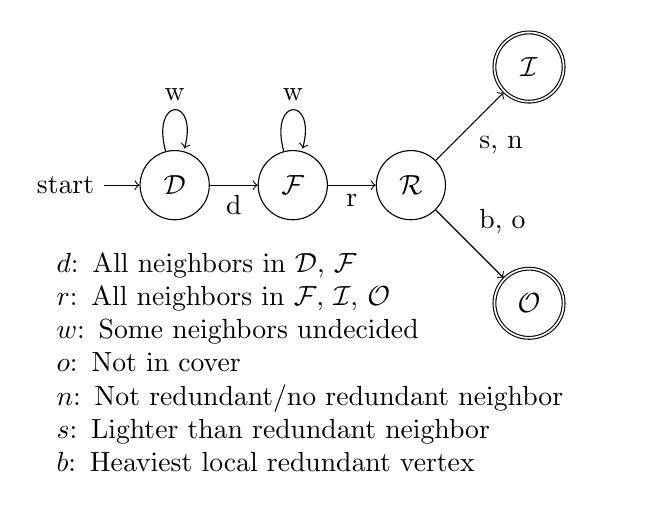
\begin{tikzpicture}
     % \draw[help lines] (0, -2) grid (5,2);
      \path [help lines] (0, -2) grid (5,2);
      \node [state, initial] (D) {\cDd};
      \node [state] (F) at (1.5, 0) {\cFd};
      \node [state] (R) at (3, 0) {\cRd};
      \node [state, accepting] (I) at (4.5, 1.5) {\cId};
      \node [state, accepting] (O) at (4.5, -1.5) {\cOd};

      \path [->] (D) edge node [below] {d} (F)
                     edge [loop above] node {w} ()
                 (F) edge node [below] {r} (R)
                     edge [loop above] node {w} ()
                 (R) edge node [above right]{b, o} (O)
                     edge node [below right]{s, n} (I);
      \node [text width=7cm] (key) at (2, -2.25) {$d$: All neighbors in \cDd, \cFd \hspace{4cm}
        $r$: All neighbors in \cFd, \cId, \cOd  \hspace{4cm}
        $w$: Some neighbors undecided  \hspace{5cm}
        $o$: Not in cover \hspace{5cm}
        $n$: Not redundant/no redundant neighbor  \hspace{4cm}
        $s$: Lighter than redundant neighbor  \hspace{4cm}
        $b$: Heaviest local redundant vertex  \hspace{4cm}};
                     
    \end{tikzpicture}
    \caption{Redundancy Checking Algorithm}
    \label{fig:red}
  \end{center}
\end{figure} 

\section{Experiments}
\label{sec:experiment}
Experiments were conducted to test algorithm performance and examine the relationship between maximizing network lifetime and minimizing vertex cover.
\subsection{Minimum Weighted Vertex Cover}
\label{sub:mwvc-exp}
Given the relationship between the target coverage and vertex cover problems, it is a reasonable hypothesis that a solution to the target coverage problem designed to maximize the lifetime of a network by reducing dependencies between covers would be a reasonable solution to the minimum weighted vertex cover. To test this hypothesis, Algorithm~\ref{alg:ldg} and Algorithm~\ref{alg:dgmm} were compared on a triangular grid.
\subsection{Experimental Design}
\label{sub:exp-design}
Random connected graphs were constructed, with the number of nodes and edges as the inputs. Nodes recieved a random weight between 100 and 1000.    

After a graph was formed, both algorithms were run on the graph and the weight of the cover output by each algorithm was recorded. The experiment was run repeatedly on graphs of 81 (9x9), 361 (19x19), and 1521(39*39) vertices. Results were averaged and can be seen in Table~\ref{tab:exp1r}.  

\subsection{Experimental Results}
\label{sub:exp-results}
\begin{table}
  \caption{Results for Experiment~\ref{sub:mwvc-exp}}
  \begin{center}
  \begin{tabular}{|l|c|c|c|}
    \hline
    &9x9&19x19&29x29\\\hline \hline
    Alg.~\ref{alg:ldg}&1738.85&8508.2&35589.3\\
    \hline
    Alg.~\ref{alg:dgmm}&1659.35&8260.8&34916.2\\
    \hline
    Total Weight&2278.95&10604.45&43572.3\\
    \hline
  \end{tabular}
  \end{center}
  \label{tab:exp1r}
\end{table}
\section{Discussion}
\label{sec:discuss}
\bibliography{vertex_bib}
\end{document}